
\section{Mobile application for data gathering and model testing}

The application was written for Android devices supporting Android 8.1 or newer. As of 2024 \cite{androidStats}, more than 93\% of Android devices should be compatible. The Android platform was chosen, as it was easier to test on and find a study group of the Android users as opposed to the iOS users (according to \cite{operatingSystemDistribution} , significantly more people in Poland, where the researchers are based in, use Android devices).

Technology used in the mobile application itself was Jetpack Compose, which is quoted by Google to be "Android’s recommended modern toolkit for building native UI" \cite{jetpackCompose}. Language used was Kotlin. Persisence was achieved by using Android Room, which provided an abstraction layer over SQLite database, which was used for data collection.

\subsection{Model View ViewModel and DataStore}

The application uses Model-View-ViewModel (MVVM) provided by Jetpack Compose design pattern to support a clear separation of concerns. 
\begin{itemize}
	\item \textbf{Model:} Data is modeled using \texttt{KeyPressEntity} class, which represents a single key press event. It includes: 
	\begin{itemize}
		\item \textbf{Key} (\texttt{String}): The key pressed by the user.
		\item \textbf{Press Time} (\texttt{Long}): The exact timestamp of the key press event.
		\item \textbf{Duration} (\texttt{Long}): The time elapsed since the last key press event.
		\item \textbf{Accelerometer Data} (\texttt{Float}): Currently unused but useful for future developing of the project. 
	\end{itemize}
	\begin{figure}[H]
		\centering
		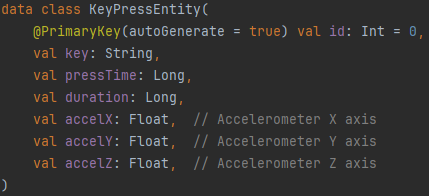
\includegraphics[width=0.8\linewidth]{images/DataModel.png}
		\caption{KeyPressEntity.kt}
		\label{fig:data_model_view}
	\end{figure}
	
	The \texttt{KeyPressEntity} is stored in a local SQLite database via Room.
	
	\item \textbf{View:} The user interface is implemented using \textbf{Jetpack Compose}, a declarative UI framework. Key components of the view contain:
	\begin{itemize}
		\item \textbf{Input Fields:} Lets users enter their credentials (University ID) and use the application for training or testing by pressing keys. 
		\item \textbf{Completion progress:} Informs users on what phase they are and displays progress of completion, linked to the \texttt{phasesCompleted} state in the \texttt{MainViewModel}.
		\item \textbf{Buttons:} Used for logging in, logging out, jumping phases and sending or downloading the data collected through training or testing stage.
	\end{itemize}
	\item \textbf{ViewModel:} This role is fulfilled by \texttt{MainViewModel}, which manages the application logic, handles interactions between the model and the view, and maintains the state of the app. \newline
	The \texttt{MainViewModel} class manages this operations through:
	\begin{itemize}
		\item \textbf{Logic Handling:} Methods such as \texttt{login()}, \texttt{logout()}, \texttt{clearDatabase()}, and \texttt{onKeyPress()} are responsible for managing user state and data.
		\item \textbf{State Management:} Stores states \texttt{isLoggedIn}, \texttt{username}, and \texttt{phasesCompleted}, which are used to dynamically update the user interface.
		\item \textbf{Data Management:} Connects with the \texttt{keyPressDao} database to process data. \texttt{onKeyPress} saves key press events into the database, \texttt{exportDataToTsv} exports the collected data into TSV files.
	\end{itemize}
\end{itemize}
In the app \textbf{DataStore} is used for storing login state and the user's ID. It has been implemented in \texttt{UserPreferences} class, and stores data such as:
\begin{itemize}
	\item \texttt{LOGGED\_IN\_KEY} - login state
	\item \texttt{USERNAME\_KEY} - user's ID.
\end{itemize}
\begin{figure}[H]
	\centering
	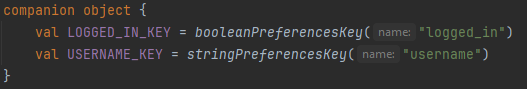
\includegraphics[width=0.8\linewidth]{images/CompanionObject.png}
	\caption{UserPreferences.kt}
	\label{fig:companion_object_view}
\end{figure}
This data is stored in the app's preferences file and can be accessed via dataStore object using:

\begin{itemize}
	\item \texttt{isLoggedIn} - returns login state as \texttt{Flow<Boolean>}
	\item \texttt{username} - returns user's ID as \texttt{Flow<String>}
	\item \texttt{setLoggedIn()} - saves login state and user's ID into DataStore
\end{itemize}

\begin{figure}[H]
	\centering
	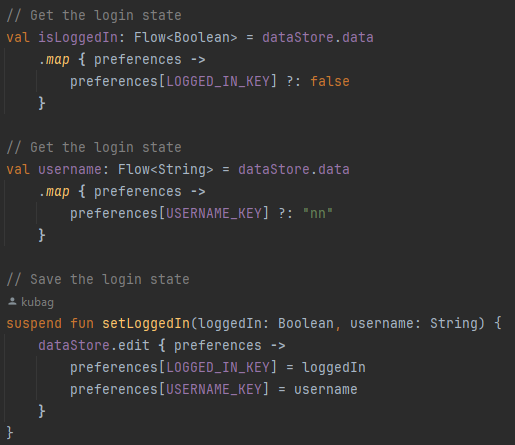
\includegraphics[width=0.8\linewidth]{images/UPFunctions.png}
	\caption{UserPreferences.kt}
	\label{fig:user_preferences_functions_view}
\end{figure}

The use of DataStore enabled the data to be stored securely, accessed and modified easily, and it is always available, which makes it a reliable and efficient way to manage user preferences and app state.

\subsection{User Interface Design}
The application design follows a minimalistic approach to make it intuitive and easy to use for everyone. 
\begin{itemize}
	\item 
	\texttt{Login Screen} \ref{fig:login_screen} \newline
	After launching the application for the first time, the user is presented with the \texttt{Login screen}. It contains \texttt{TextInput} field for entering the university ID, which was evenly distributed among contributors to simplify testing, and the \texttt{Log in} button which stores the ID and navigates the user to the \texttt{Home Screen}.
	\item 
	\texttt{Home Screen} \ref{fig:home_screen} \newline
	The home screen displays three buttons and a simple note explaining what the user should do. The \texttt{Logout} button navigates back to the \texttt{Login Screen}, while two other buttons lead to either testing or training screens.
	\item 
	\texttt{Training Screen} \ref{fig:training_screen} \newline
	The training screen is designed for collecting data for training purposes. It includes \texttt{TextInput} field for typing user input, a \texttt{Button} to proceed to the next phase, and \texttt{Text} indicators showing how many chars are needed to complete the phase (300 each phase) and how many phases remain (5 phases in total) to complete the process of collecting training data. Additionally, there are two notes instructing the user to maintain the writing style throughout the whole process and to change the position after each phase while writing (explained in subsection~\ref{sec:data_collection}). \newline
	To ensure that typing is done in the most natural way, the default android keyboard is used. 
	\item 
	\texttt{Testing Screen} \ref{fig:testing_screen} \newline
	The testing screen includes \texttt{TextInput} field for typing the test input, a \texttt{Button} that sends the input to the server and stores it locally, and \texttt{Text} indicators showing how many characters need to be written (in this case, 100). After fulfilling the requirements, the user sends their input to the server, followed by the presentation of the recognition rate percentage on a circular progress bar and a message indicating whether the model recognised the user or not. 
\end{itemize}


\begin{figure}[H]
	\centering
	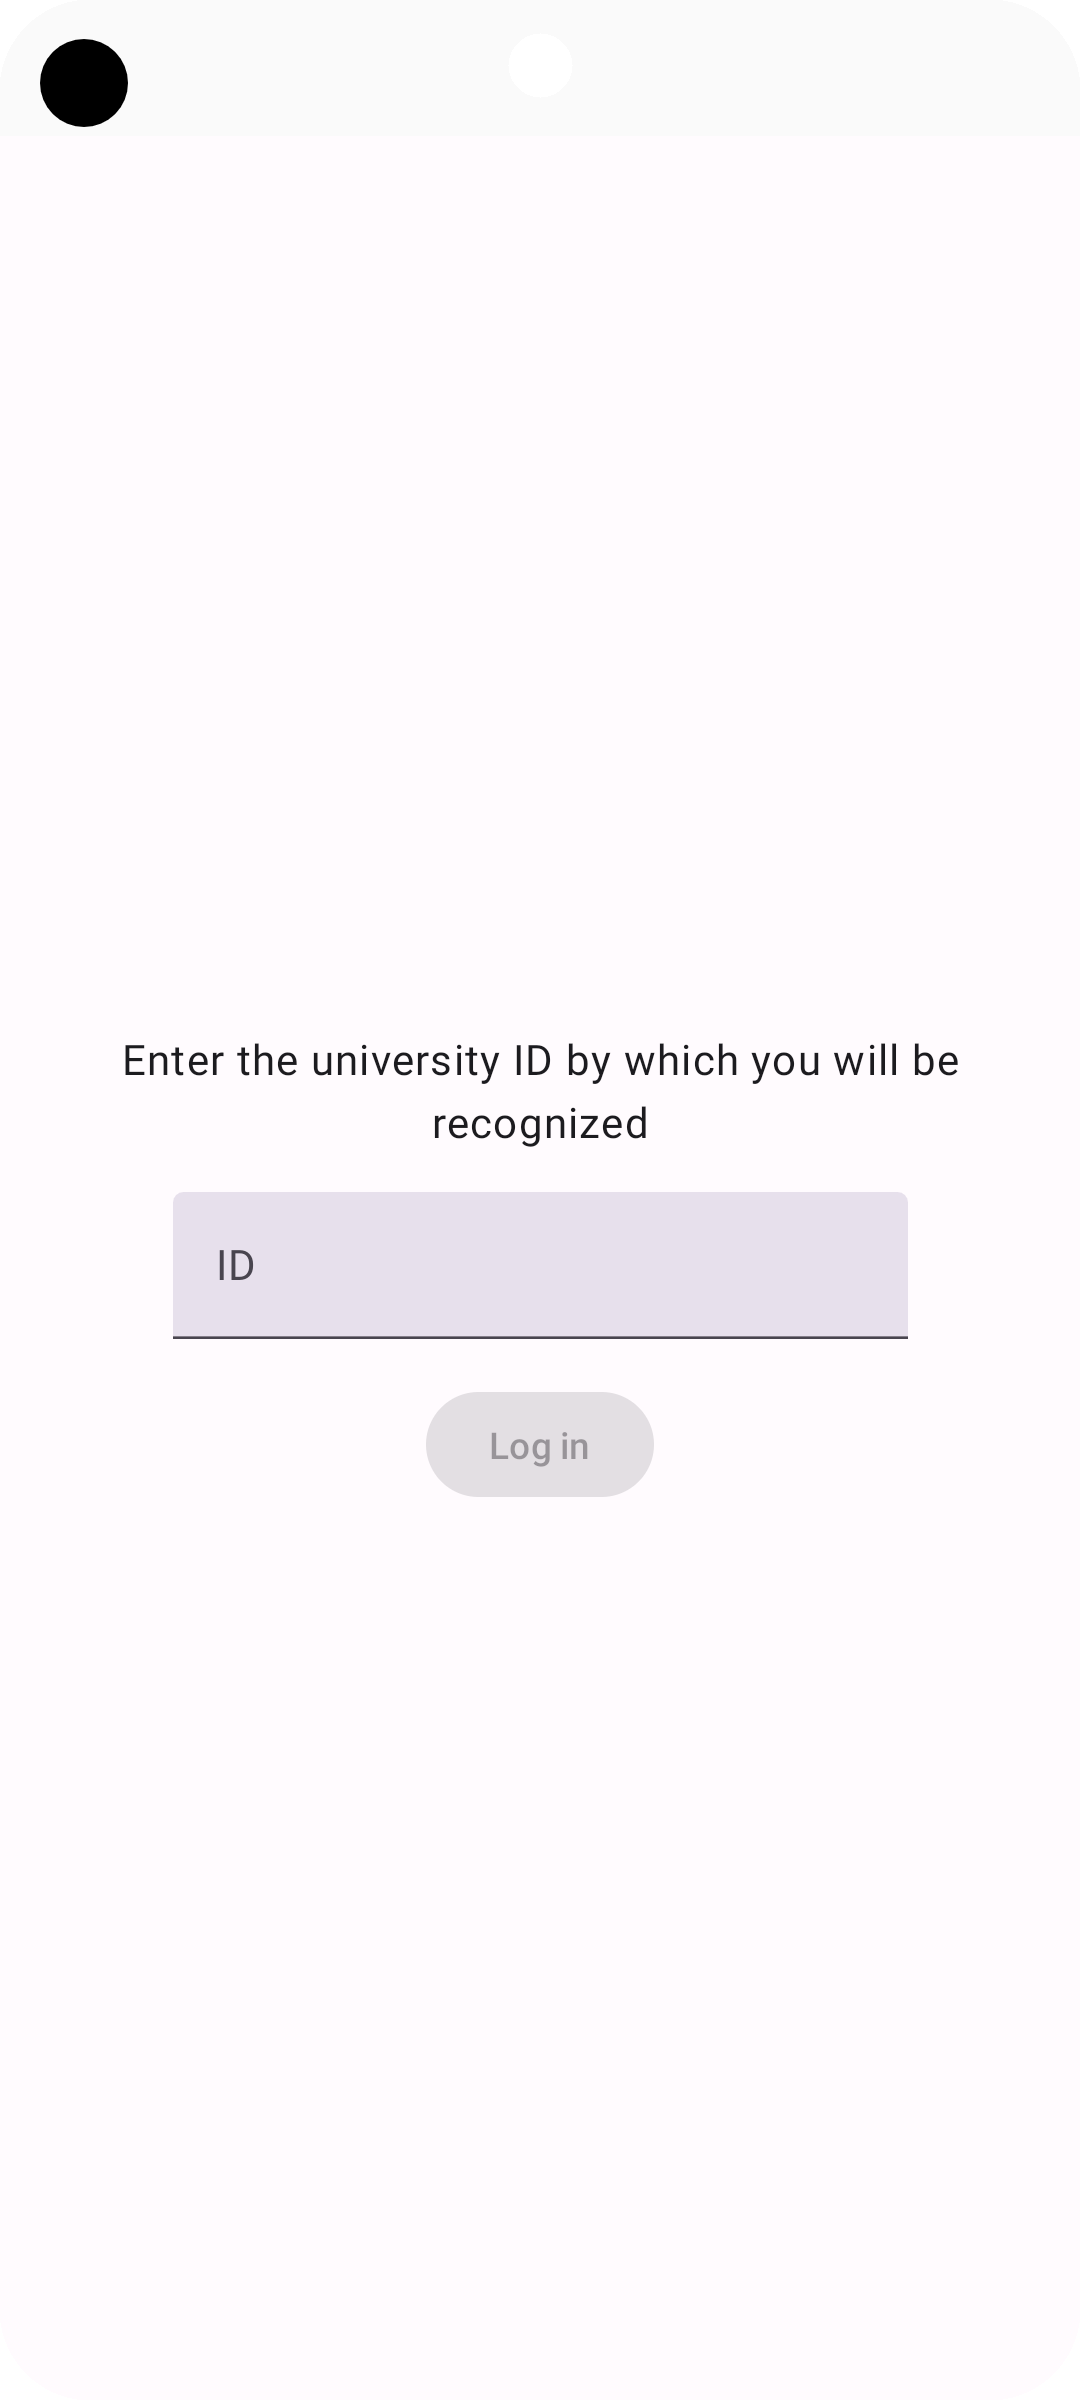
\includegraphics[width=0.32\linewidth]{images/login_screen.png}
	\caption{Login screen}
	\label{fig:login_screen}
\end{figure}

\begin{figure}[H]
	\centering
	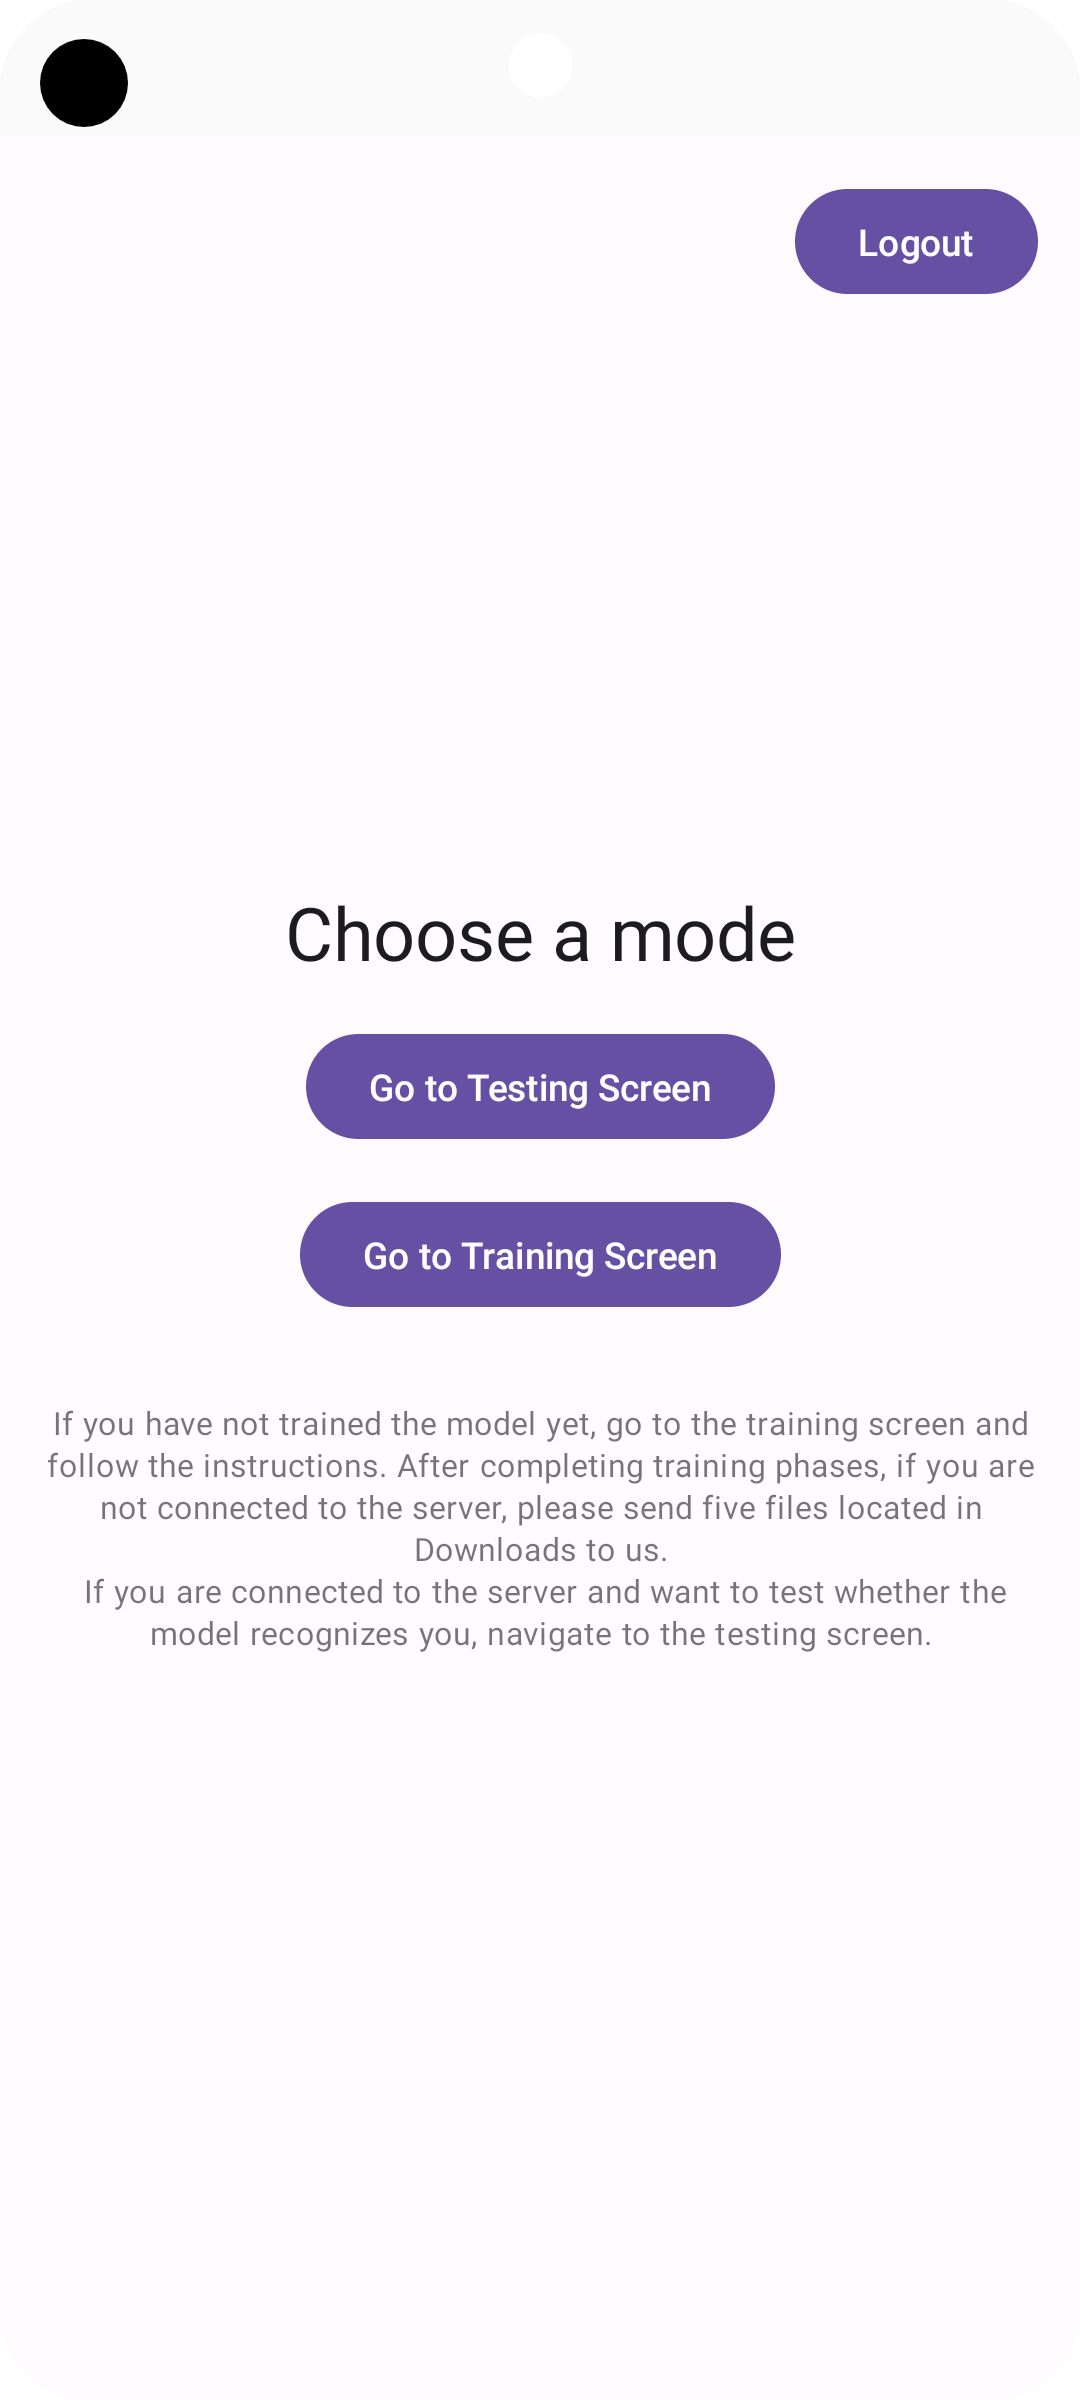
\includegraphics[width=0.32\linewidth]{images/home_screen.png}
	\caption{Home screen}
	\label{fig:home_screen}
\end{figure}

\begin{figure}[H]
	\centering
	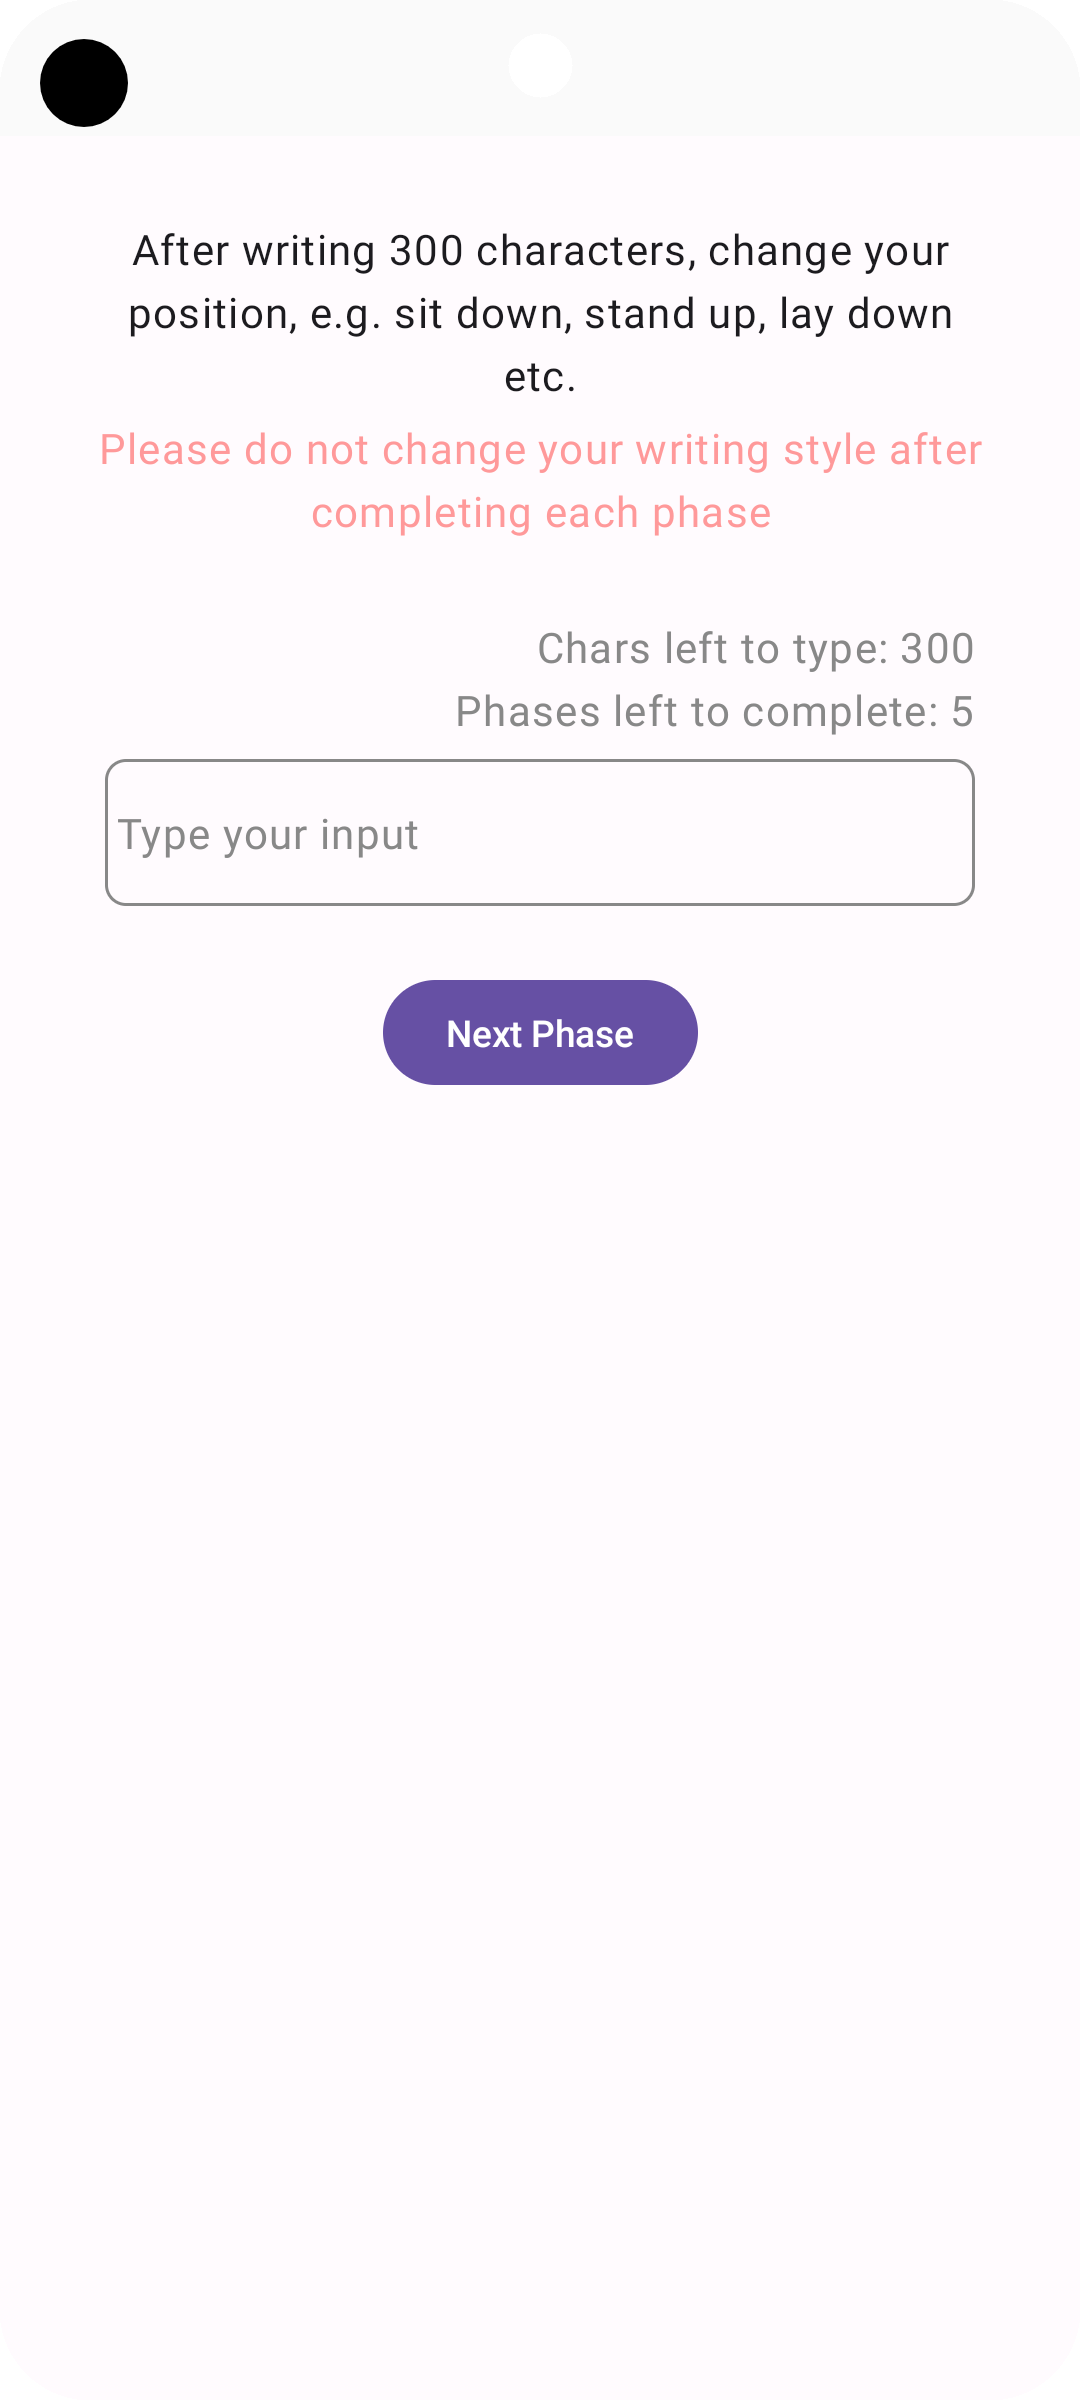
\includegraphics[width=0.32\linewidth]{images/training_screen.png}
	\caption{Training screen}
	\label{fig:training_screen}
\end{figure}

\begin{figure}[H]
	\centering
	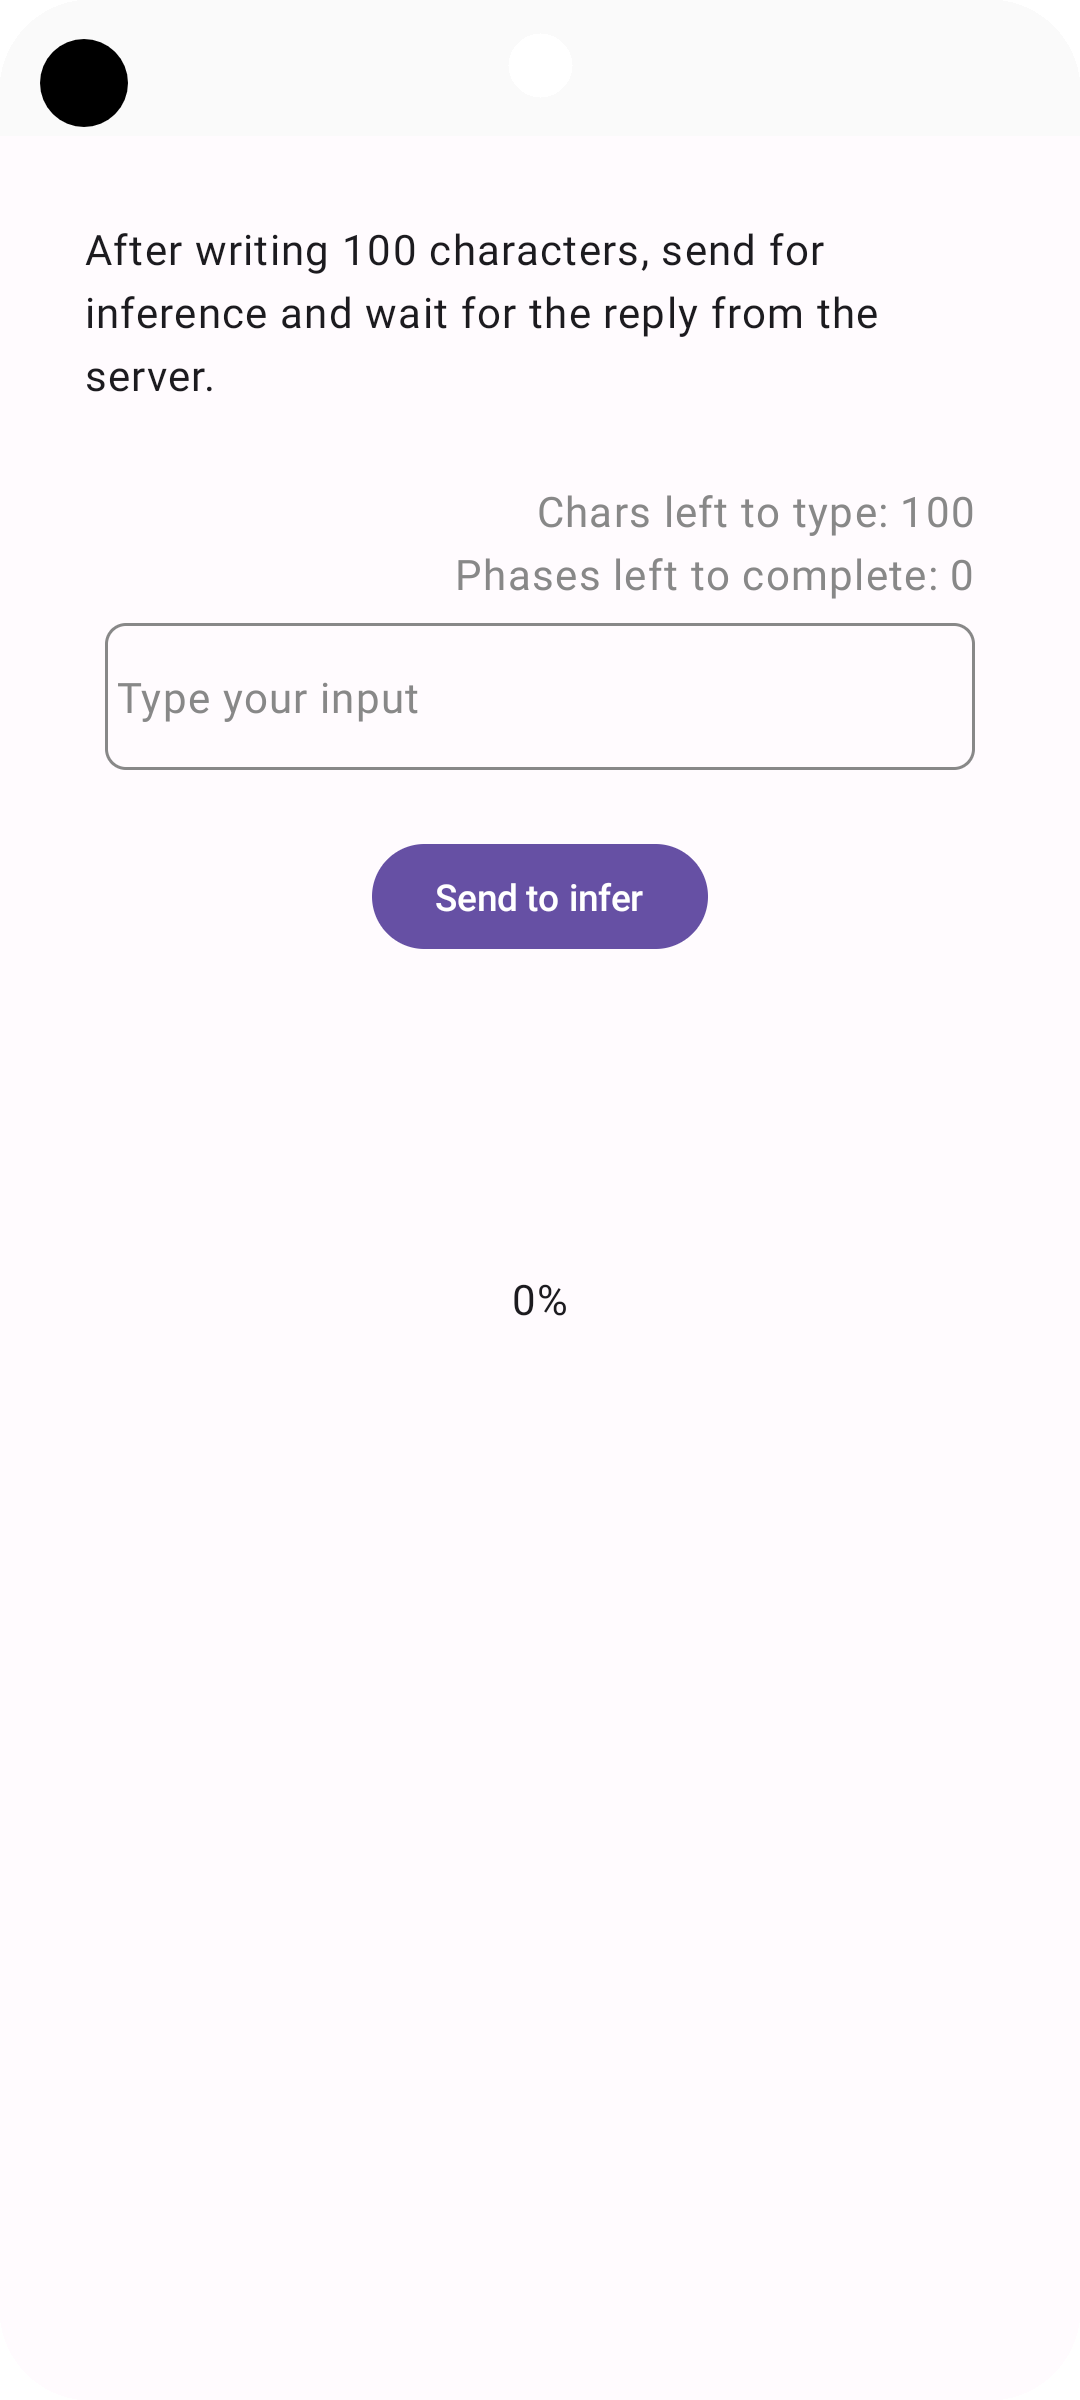
\includegraphics[width=0.32\linewidth]{images/testing_screen.png}
	\caption{Testing screen}
	\label{fig:testing_screen}
\end{figure}

\subsection{Data Collection Process}
\label{sec:data_collection}
Data collection occurs in two stages, training and testing
\begin{itemize}
	\item 
	Training data collection begins on the \texttt{Training Screen} \ref{fig:training_screen}, where the user is asked to input meaningful sentences. The process consists of 5 phases. Each phase requires the user to type 300 characters. Once the requirement is met, the user progresses to the next phase until all 5 phases are completed (1500 characters in total). Additionally, there is a note instructing the user to maintain a consistent writing style throughout all phases. Also the user is asked to change their position after each phase while writing. This is important for accelerometer data collection (which is not used at the moment), as it helps exclude situations where the phone is lying on the table or being held in an atypical way.  
	\item 
	Testing data collection takes place on the \texttt{Testing Screen} \ref{fig:testing_screen}, where the user is required to write 100 characters, again in meaningful sentences. Once this is done, the testing phase is complete.
\end{itemize}
After each phase, the collected data is saved in a \texttt{.tsv} file, sent to the server, and stored locally in the phone's downloads directory. The \texttt{exportDataToTsv} \ref{fig:export_data_code} function from \texttt{MainViewModel.kt} handles the export of key press data. \newline Firstly it retrieves latest key press events using the \texttt{keyPressDao.getNLatestKeyPresses} method, converting the data into a \texttt{.tsv} format using the \texttt{keyPressesToTsv} function. \newline
Depending on which phase the user is in, the function determines the different type of operation to perform.
\begin{itemize}
	\item 
	If the user is in inference phase, the data will be used for inference.
	\item 
	If the user is in training phase, the data will be used for training.
	\item 
	If the number of completed phases exceeds the required amount, the function exits without performing any other action.
\end{itemize}

After processing data \texttt{saveTsvToDownloads} stores data locally, and \texttt{sendTsvToFastApi} sends data to the server (An example of the \texttt{.tsv} file containing the saved data is shown in Figure \ref{fig:tsv_example}). The username, and the relevant phase is included in the file name. \newline
This function ensures that after each phase of training and testing, the data is collected, stored, and transmitted.

\begin{figure}[H]
	\centering
	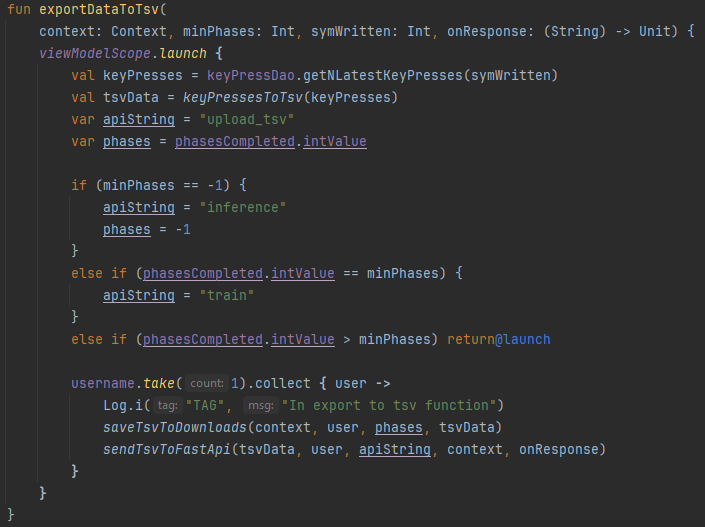
\includegraphics[width=0.8\linewidth]{images/ExportData.png}
	\caption{MainViewModel.kt}
	\label{fig:export_data_code}
\end{figure}

\begin{figure}[H]
	\centering
	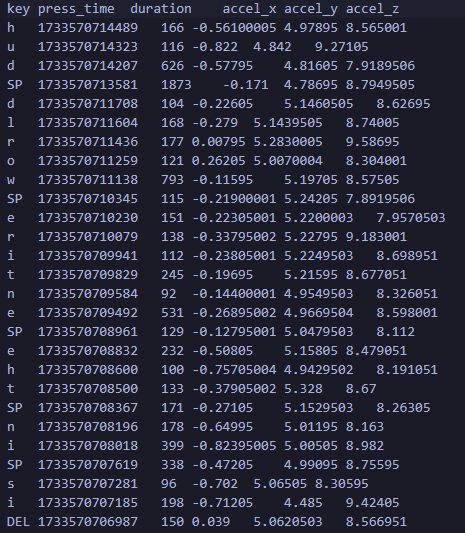
\includegraphics[width=\textwidth]{images/data_example.png}
	\caption{An example of the \texttt{.tsv} file containing saved data.}
	\label{fig:tsv_example}
\end{figure}

\subsection{Communication with the server}

The application communicates with the server using an HTTPS connection.
\begin{itemize}
	\item 
	\textbf{Server URL and Request Structure}
	\begin{itemize}
		\item 
		The server is accessed via an HTTPS endpoint. The base URL is defined as \newline \texttt{https://192.168.1.100:8000}.
		\item 
		The API endpoint is dynamically created with the use of a route and query parameters to the base URL. For example, the endpoint for sending data contains the username as a query parameter: \newline
		\texttt{https://192.168.1.100:8000/<api\_string>?username=<username>}
		\item 
		The data is sent using the POST method.
	\end{itemize}
	\item
	\textbf{Data format} \newline
	The data sent to the server is stored in \texttt{.tsv} (tab-separated values) file, containing headers and the detailed information about key presses.
	\item 
	\textbf{Secure Connection Setup}
	\begin{itemize}
		\item 
		The application uses \texttt{OkHttpClient} library for handling network requests.
		\item 
		A \texttt{.cert} certificate (stored in \texttt{res/raw/cert}) is used to establish a secure and trustworthy \texttt{SSL/TLS} connection.
	\end{itemize}
	\item 
	\textbf{Sending request}
	\begin{itemize}
		\item 
		Requests are executed asynchronously using the \texttt{enqueue} method.
		\item 
		If successful, the server's response is processed, and the application displays the result to the user.
		\item 
		On failure, the error is logged, and the user is notified.  
	\end{itemize}
	\item 
	\textbf{Error Handling}
	\begin{itemize}
		\item 
		Network errors (e.g., problems with connection) and server errors are logged for easier debugging.
		\item 
		A callback mechanism is used to provide feedback to the user. 
	\end{itemize}
	
	
\end{itemize}


\subsection{Testing screen}

Testing screen... \myworries{TODO Add screenshot and write sth about testing the model, how the \% work and so on}